\section{Смешанный языка Дика}\label{section:dyck_1_1}

\subsection{Алгоритм для смешанного языка Дика}

Смешанный язык Дика $\cool{D}_i \odot \cool{D}_j$ является пересечением двух КС языков, а именно, 
$\cool{D}_i \odot \cool{D}_j = L_1 \cap L_2$, где 
$L_1 \colon S_1 \to S_1 S_1~|~(_1 S_1 )_1~|~ \dots (_i S_1 )_i ~|~ \eps ~|~ [_1 ~|~ ]_1 ~|~ \dots ~|~ [_j ~|~ ]_j$ и 
$L_2 \colon S_2 \to S_2 S_2~|~[_1 S_2 ]_1~|~ \dots [_j S_2 ]_j ~|~ \eps ~|~ (_1 ~|~ )_1 ~|~ \dots ~|~ (_i ~|~ )_i$ 
(то есть двух языков Дика, которые игнорируют скобки второго типа). 

Однако КС-языки не замкнуты относительно пересечения: при нём получается конъюнктивный язык~\cite{Okhotin01}, задача достижимости для которого является алгоритмически неразрешимой~\cite{Hellings14}. Более того, она неразрешима уже для языка $\cool{D}_2 \odot \cool{D}_2$ даже на двунаправленных графах~\cite{Li21}. 

Однако задача достижимости для языка $\cool{D}_1 \odot \cool{D}_1$ на двунаправленных графах вполне разрешима, причём за полиномиально время.

В этой главе будет приведён улучшение алгоритма Ли и др.~\cite{Li21} решения этой задачи, основанное на идее пересечения языков.

\begin{note}\label{fact:intersection}

  Здесь и далее будем считать, что первый язык Дика~--- язык круглых ПСП ($\cool{D}_p \colon S \to SS~|~(S)~|~\eps$), второй~--- язык квадратных ПСП ($\cool{D}_b \colon T \to T~|~[T]~|~\eps$).
\end{note}

Заметим, что слово принадлежит $\cool{D}_p \odot \cool{D}_b$, тогда и только тогда, когда на любом его префиксе баланс обоих типов скобок неотрицателен, а конечный баланс равен нулю. Баланс строки будем записывать как $(p, b)$, где $p$~--- баланс круглых скобок, а $b$~--- квадратных.

Для решения понадобится следующий вспомогательный факт:

\begin{lemma}{Ли и др.~\cite{Li21}}\label{lm:dyck_6v}
  В двунаправленном графе, если между парой вершин $(u, v)$ существует какой-то $\cool{D}_1 \odot \cool{D}_1$ путь, то существует и такой путь, на котором в любой момент времени вложенность хотя бы одного типа скобок не превышает $6 |V|$.
\end{lemma}

\begin{figure}[h]
  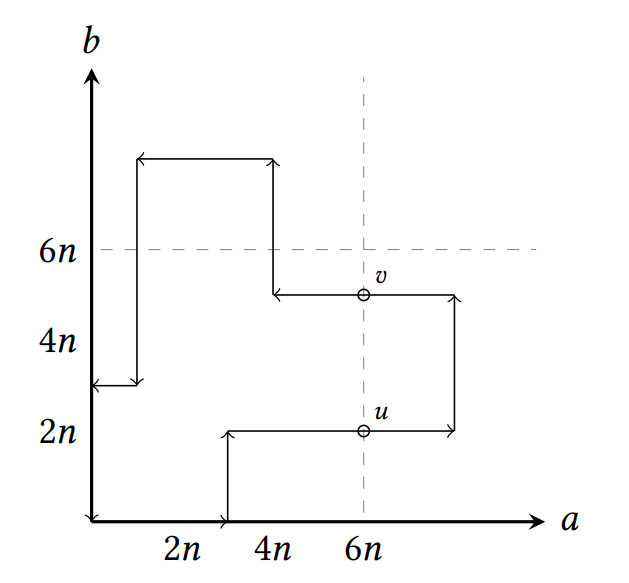
\includegraphics[width=0.75\linewidth]{img/6n_6n_path}
  \caption{Путь в координатах баланса}
  \label{img:6v_path}
\end{figure}

\TODO: картиночька

Нарисуем~(рис.~\ref{img:6v_path}) такой (как в утверждении леммы~\ref{lm:dyck_6v}) путь на плоскости, где первая координата~--- баланс круглых скобок, вторая~--- баланс квадратных (т.е. просто $p$ и $b$). Тогда во-первых, весь путь будет проходить в первой четверти. Во-вторых, он не будет заходить (найдётся такой, что не будет заходить, и мы ищем именно его) в сектор $[6|V|+1, +\oo) \times [6|V|+1, +\oo)$
    
То есть путь можно искать следующего вида: он в основном проходит внутри квадрата $[0, 6|V|] \times [0, 6|V|]$, иногда выходя из него, но только по одной координате (т.е. либо в сектор $[0, 6|V|] \times [6|V| + 1, +\oo)$, либо в сектор $[6|V| + 1, +\oo) \times [0, 6|V|]$).

Тогда можно искать отдельно две эти сущности: куски путей внутри квадрата $[0, 6|V|] \times [0, 6|V|]$, и куски путей снаружи.

Вооружившись этим знанием, построим алгоритм:

\begin{enumerate}
    \item {\bf Часть пути, лежащая в квадрате $\mathbf{[0, 6|V|] \times [0, 6|V|]}$}

    Внутри квадрата ограничена вложенность обоих типов скобок. Помним из прошлой главы (замечание~\ref{fact:regular_cfpq}), что в случае ограниченной вложенности язык получается регулярным. Строим автоматы для таких регулярных языков: $\cool{D}_p^{6|V|}$ и $\cool{D}_b^{6|V|}$, оба размера $\O(n)$.

    Пересекая оба этих языка и входной граф получаем автомат, состояние в котором~--- тройка $\q{v, p, b}$ (вершина и два баланса). Размер автомата: $\O(|V|^3)$ вершин, $\O(|E||V|^2)$ рёбер.

    Также в этом автомате нужно провести $\eps$-рёбра, соответствующие путям, выходящим за границы квадрата. Такие пути идут из состояния $(u, 6|V|, b_1)$ в состояние $(v, 6|V|, b_2)$ (и аналогично для другого типа скобок). Таких рёбер может быть столько, сколько есть различных пар $(u, b_1)$/$v, b_2$, то есть $\O(|V|^4)$.

    % Макс <3
    \begin{figure}[h]
      \begin{tikzpicture}
        \node[state, initial, accepting](n0) {$0$};
        \node[state, right=of n0](n1) {$1$};
        \node[state, right=of n1](n2) {$2$};
        \node[state, right=6em of n2](n3) {$3$};
        \node[state, right=6em of n3](n4) {$6|V|$};

        \foreach \y [evaluate=\y as \ny using int(\y+1)] in {0,1} {
          \draw (n\y)  edge[bend left=15] node[above] {\tt (} (n\ny);
          \draw (n\ny) edge[bend left=15] node[below] {\tt )} (n\y);
        }

        \foreach \y [evaluate=\y as \ny using int(\y+1)] in {2,3} {
          \draw (n\y)  edge[bend left=15] node[above] {\tt (} (n\ny);
          \draw (n\ny) edge[bend left=15] node[below] {\tt )} (n\y);
        }

        \foreach \y  in {0,1,2,4} {
          \draw (n\y) edge[loop above] node{\tt [,]} (ny);
        }

        \node [thick, fill=white, shape=rectangle, minimum width=6em, minimum height=4em, anchor=center] at ([yshift=0em]n3) {$\dots$};
      \end{tikzpicture}
      \caption{Автомат для языка $\cool{D}_p^{6|V|}$}
      \label{img:dyck_6n_dfa}
    \end{figure}

    После этого нужно решить задачу достижимости для полученного графа-автомата. Покажем, что он получается неориентированным: из-за двунаправленности графа ребро $(u, b, p) \to (v, b+1, p)$ существует тогда и только тогда, когда и обратное ему. То же и с $\eps$-рёбрами: если есть путь, с балансом $(0, j-i)$, то есть и путь в обратную сторону с балансом $(0, i-j)$.

    В неориентированном графе выделяем компоненты связности, теперь из вершины $u$ есть $\cool{D}_p \odot \cool{D}_p$-путь, если $(u, 0, 0)$ и $(v, 0, 0)$ лежат в одной компоненте.

    Итого, эта часть алгоритма работает за dfs по графу-произведению, то есть за $\O(|V|^4)$.

    \item {\bf Часть пути, лежащая в $\mathbf{[0, 6|V|] \times [6|V| + 1, +\oo)}$}

    Хотим найти все пути вида $(u, 6|V|, b_1) \path (v, 6|V|, b_2)$, то есть пути, образующие правильные круглые ПСП, а по квадратным дающие разницу балансов $b_2 - b_1$. При этом квадратный баланс не должен подниматься выше $6|V|$ и опускаться ниже 0 (то есть важно его стартовое значение).

    Будем решать отдельно для каждого стартового квадратного баланса $b_1$. Снова делаем это через пересечения языков. Первый~--- входной граф, второй~--- круглые ПСП (язык $\cool{D}_p$ из~\ref{fact:intersection}). Третий~--- регулярный язык, считающий квадратный баланс $\cool{D}_b^{b_1, 6|V|}$, его единственное отличие от языков в прошлом пункте в том, что баланс может опускаться не до 0, а до $-b_1$ (и подниматься до $6|V| - b_1$, а не до $6|V|$).

    Пересекаем языки в хитром порядке: сначала первый и третий (т.е. входной граф и регулярный язык), получим опять-таки граф пар $(v, p)$~--- вершина и круглый баланс~--- на $\O(|V|^2)$ вершинах и $\O(|V||E|)$ рёбрах. Дальше нужно пересечь его со вторым языком, который просто является языком Дика, то есть решить для него задачу Диковой достижимости.

    Заметим, что граф $L(G) \cap \cool{D}_b^{b_1, 6|V|}$ получится также двунаправленным:

    \vspace{-\topsep}
    \begin{itemize}
      \setlength\itemsep{-0.1em}   
      \item $u \xrightarrow{[} v$ в $G$ $\SO$ рёбра $\q{u, b} \xrightarrow{\eps} \q{v, b+1}$ в пересечении
      \item $u \xrightarrow{]} v$ в $G$ $\SO$ рёбра $\q{u, b} \xrightarrow{\eps} \q{v, b-1}$ в пересечении
      \item $u \xrightarrow{[} v$ $\EQ$ $v \xrightarrow{]} u$, так что $\eps$-рёбра двунаправлены
      \item $u \xrightarrow{(} v$ в $G$ $\SO$ рёбра $\q{u, b} \xrightarrow{(} \q{v, b}$ в пересечении
      \item $u \xrightarrow{)} v$ в $G$ $\SO$ рёбра $\q{u, b} \xrightarrow{)} \q{v, b}$ в пересечении
      \item $u \xrightarrow{(} v$ $\EQ$ $v \xrightarrow{)} u$, так что $($ и $)$-рёбра также двунаправлены
    \end{itemize} 

    Задача Диковой достижимости на двунаправленных графах решается за время $\O(|V| \alpha(|V|) + |E|)$~\cite{Chatterjee17} (в нашем случае, получится $\O(|V||E|)$. Решаем её, теперь путь $(u, 6|V|, b_1)~\path~(v, 6|V|, b_2)$ существует тогда и только тогда, когда $(v, b_2 - b_1)$ Диково достижимо из $(u, 0)$ в полученном графе.

    Получаем алгоритм за $\O(|V||E|)$ для каждого $b_1$, итого $\O(|V|^2 |E|)$.

\end{enumerate}

\begin{theorem}
  Для задачи $\cool{D}_1 \odot \cool{D}_1$-достижимости существует алгоритм с временем работы $\O(|V|^4)$.
\end{theorem}

\subsection{Выводы и результаты по главе}

В данной главе был приведена модификация алгоритма Ли и др.~\cite{Li21} решения задачи достижимости для смешанного языка Дика $\cool{D}_1 \odot \cool{D}_1$ на двунаправленных графах, в которой применялась идея пересечения языков: входной граф пересекался с двумя языками Дика, которые в обоих случая были ограничены так, что хотя бы один из них становился регулярным.

% 
\includegraphics[width=0.75\linewidth]{img/conclusion_cat}

% \TODO{}